\chapter{Capa ETL con Apache Hop}
\label{chap:desarrollo_etl}

\lettrine{E}{l} éxito de un sistema de Business Intelligence radica en la calidad, consistencia y fiabilidad de sus datos. En esta fase central del proyecto se ha utilizado \textbf{Apache Hop}, una plataforma moderna e innovadora de orquestación y procesamiento de datos basada en metadatos, para diseñar e implementar los procesos de Extracción, Transformación y Carga (ETL).

Este capítulo detalla la arquitectura de los flujos de datos (\textit{Pipelines}) y de trabajo (\textit{Workflows}) desarrollados en Apache Hop para poblar el Datamart y calcular los índices de riesgo de abandono. El entorno se ejecuta sobre la imagen Docker oficial, conectándose mediante JDBC a las bases de datos origen (\textit{conn\_source}, solo lectura) y destino (\textit{conn\_dwh}, lectura/escritura).

\section{Análisis de pipelines}

\subsection{Volcado a staging (\textit{extract\_all\_to\_staging.hpl})}
Para no sobrecargar la base de datos transaccional durante los cruces analíticos, el primer paso es clonar las tablas de producción al esquema intermedio \textit{raw} (Staging Area). El pipeline establece 14 hilos independientes que extraen datos de forma incremental usando el parámetro \textit{\$\{CURSO\_ACTUAL\}}, permitiendo recargas históricas completas si el parámetro se omite. 

Una decisión clave es la \textbf{ausencia de claves foráneas} en el esquema destino \textit{raw}, lo que permite a Hop paralelizar la inserción masiva de todas las entidades simultáneamente sin generar bloqueos lógicos por dependencias (ver figura \ref{fig:extract_all_to_staging}).

\begin{figure}[htbp]
    \centering
    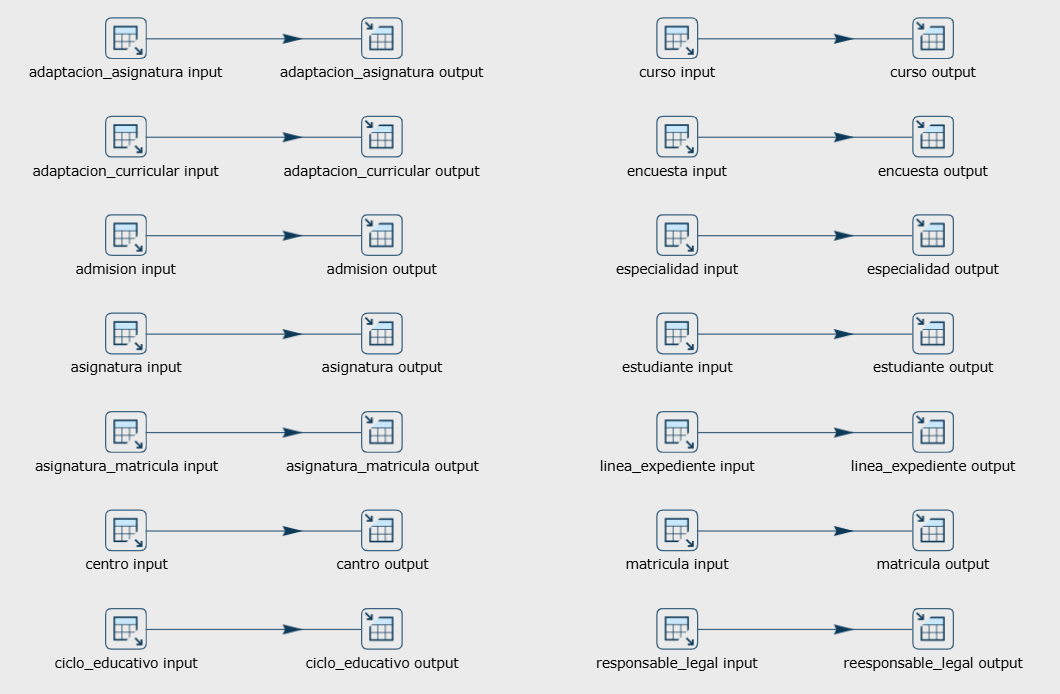
\includegraphics[width=0.85\textwidth]{imaxes/extract_all_to_staging.png}
    \caption{Flujo del pipeline \textit{extract\_all\_to\_staging.hpl}.}
    \label{fig:extract_all_to_staging}
\end{figure}

\subsection{Dimensión de demografía familiar}

El núcleo de las reglas de negocio reside en este pipeline, cuya misión es ingerir datos brutos de encuestas y construir una dimensión de baja cardinalidad consolidando perfiles de riesgo socioeconómico (ver figura \ref{fig:dim_demografia_familiar}).

El flujo encadena operaciones matemáticas para derivar ratios (como la renta por unidad de consumo o la ratio de ordenadores por hijo) y nodos \textit{NumberRange} para discretizar estas variables continuas en bandas analíticas fijas (ej. renta "Baja", "Media/Alta"). Mediante transformaciones \textit{ValueMapper}, se asignan pesos numéricos de riesgo a cada factor (ej. renta muy baja suma 15 puntos, falta de internet suma 3 puntos). Una fórmula final consolida la puntuación total de riesgo.

Para optimizar la cardinalidad, un paso de ordenación con filtrado de filas únicas (\textit{unique\_rows=Y}) descarta duplicados en memoria, garantizando que el Datamart solo almacene las combinaciones únicas de factores socioeconómicos antes de asignar la clave subrogada \textit{id\_demografia\_familiar}.

\begin{figure}[htbp]
    \centering
    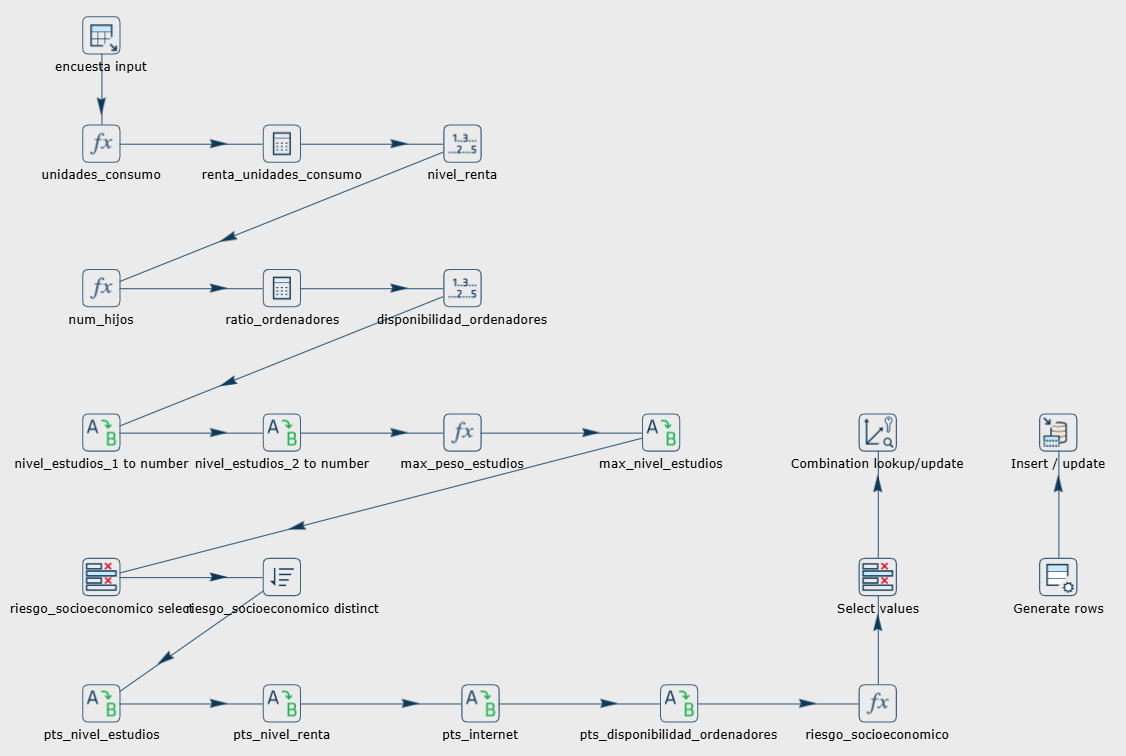
\includegraphics[width=0.85\textwidth]{imaxes/dim_demografia_familiar.png}
    \caption{Flujo del pipeline \textit{dim\_demografia\_familiar.hpl}.}
    \label{fig:dim_demografia_familiar}
\end{figure}

\subsection{Dimensión de estudiante}

La casuística de un estudiante no es estática: puede cambiar de domicilio o tutor legal a lo largo de los años. Para no perder el contexto socioeconómico histórico asociado a calificaciones pasadas, este pipeline implementa un algoritmo SCD (Slowly Changing Dimension) Tipo 2 (ver figura \ref{fig:dim_estudiante}).

Tras cruzar los datos del estudiante y sus tutores legales, y aplicar transformaciones de limpieza de cadenas (separación de direcciones, casteo numérico de códigos postales), el flujo utiliza el nodo \textit{Dimension lookup/update} configurado para rastrear el ciclo de vida del \textit{num\_expediente} (clave natural). La configuración micro-gestiona las actualizaciones campo a campo:
\begin{itemize}
    \item \textbf{\textit{Punch through} (SCD Tipo 1):} Correcciones en datos estáticos (\textit{dni}, \textit{nombre}) sobrescriben el valor en todas las versiones históricas.
    \item \textbf{\textit{Insert} (SCD Tipo 2):} Mutaciones en el contexto socioeconómico (\textit{cod\_responsable}, \textit{ciudad}) congelan la fila antigua (estampando \textit{date\_to}) e insertan una nueva versión activa con nuevo \textit{id\_estudiante}.
    \item \textbf{\textit{Update}:} Cambios en datos secundarios (\textit{email}) actualizan la fila activa sin generar nueva versión histórica.
\end{itemize}

\begin{figure}[htbp]
    \centering
    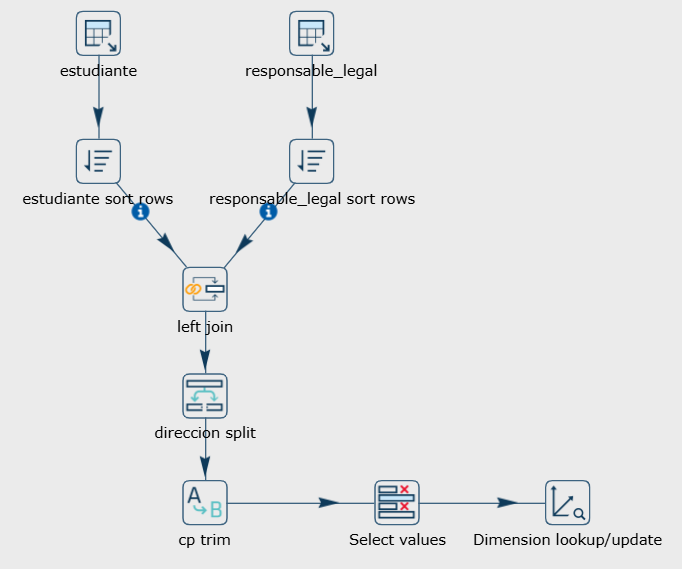
\includegraphics[width=0.85\textwidth]{imaxes/dim_estudiante.png}
    \caption{Flujo del pipeline \textit{dim\_estudiante.hpl}.}
    \label{fig:dim_estudiante}
\end{figure}

\subsection{Dimensión de tiempo}

Este sistema requiere una dimensión de tiempo académica que categorice momentos evaluativos ("Curso 2023-2024, 1ª Evaluación"). El pipeline infiere automáticamente estas temporalidades desde los registros transaccionales de matrículas y expedientes (Figura \ref{fig:dim_tiempo}).

Tras cruzar los datos y extraer el dominio temporal real filtrando los pares únicos de curso y evaluación, un nodo \textit{FilterRows} analiza léxicamente el texto buscando la subcadena "Final" para bifurcar el flujo e inyectar una constante booleana (\textit{is\_final}). La persistencia emplea un patrón híbrido: un nodo \textit{Combination lookup/update} inserta la fila generando la clave \textit{id\_tiempo}, seguido síncronamente de un paso \textit{Update} que persiste el atributo \textit{is\_final}.

\begin{figure}[htbp]
    \centering
    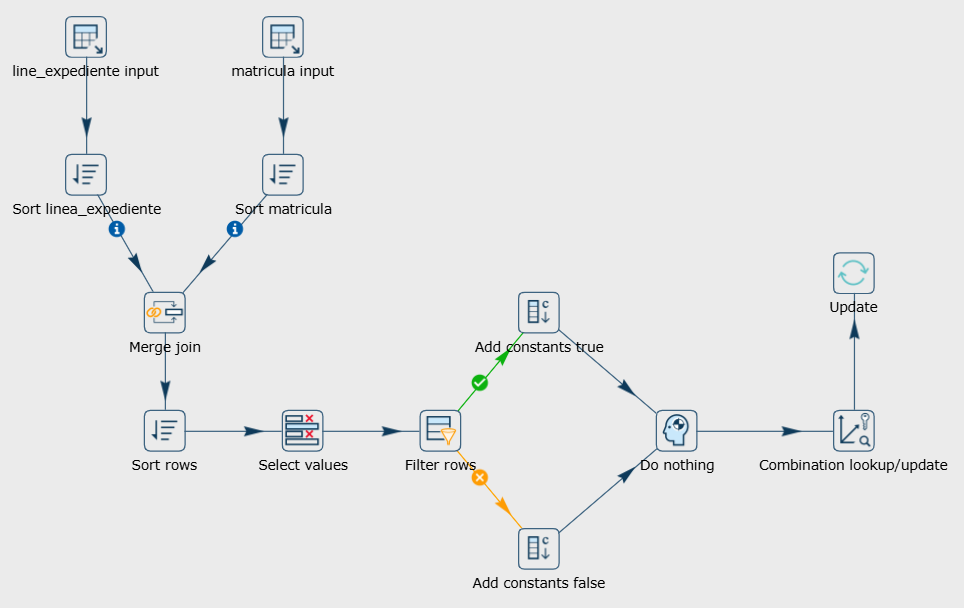
\includegraphics[width=0.85\textwidth]{imaxes/dim_tiempo.png}
    \caption{Flujo del pipeline \textit{dim\_tiempo.hpl}.}
    \label{fig:dim_tiempo}
\end{figure}

\subsection{Dimensión de asignatura}

El modelo origen de asignaturas presenta una arquitectura relacional normalizada en "Copo de Nieve". Para modelarlo en el Data Warehouse bajo un esquema en Estrella óptimo para lectura, este pipeline colapsa jerarquías relacionales en una única fila dimensional mediante nodos \textit{DBLookup} encadenados que recorren las claves foráneas hacia arriba, recuperando información del curso, la especialidad y el ciclo educativo antes de generar la clave \textit{id\_asignatura} (ver figura \ref{fig:dim_asignatura}).

\begin{figure}[htbp]
    \centering
    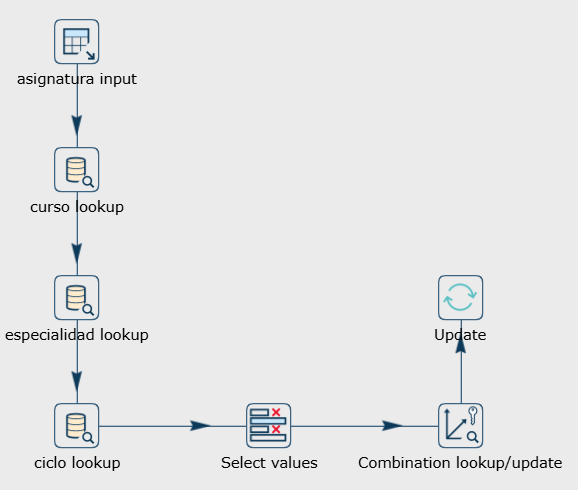
\includegraphics[width=0.85\textwidth]{imaxes/dim_asignatura.png}
    \caption{Flujo del pipeline \textit{dim\_asignatura.hpl}.}
    \label{fig:dim_asignatura}
\end{figure}

\subsection{Dimensión de curso}

Esta dimensión almacena los metadatos del curso y calcula la edad teórica esperada del alumno, clave para medir el desfase de edad en la tabla de hechos. Un nodo \textit{ValueMapper} inyecta la edad base de acceso al ciclo ("PRI" $\rightarrow$ 5, "ESO" $\rightarrow$ 11), y un \textit{Calculator} le suma el ordinal del curso para consolidar la \textit{edad\_ideal} (ver figura \ref{fig:dim_curso}).

\begin{figure}[htbp]
    \centering
    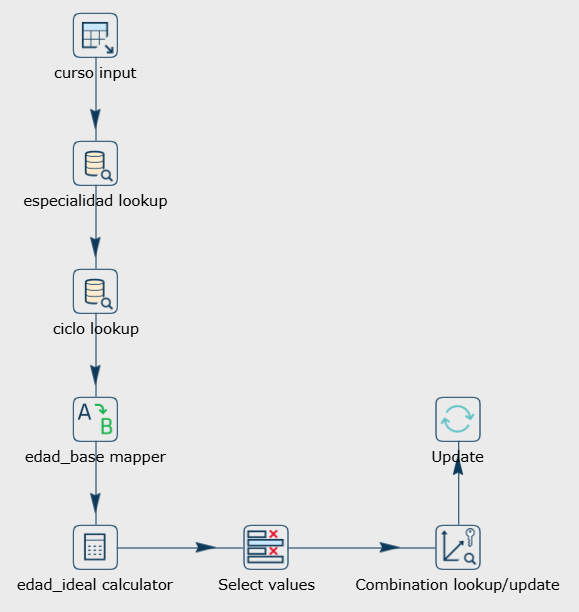
\includegraphics[width=0.85\textwidth]{imaxes/dim_curso.png}
    \caption{Flujo del pipeline \textit{dim\_curso.hpl}.}
    \label{fig:dim_curso}
\end{figure}

\subsection{Dimensión de adaptación}

El registro transaccional de adaptaciones suele ser texto libre. Este pipeline actúa como motor de extracción de reglas clínicas mediante expresiones regulares (\textit{RegexEval}), clasificando el texto en discapacidades fisiológicas/neuropsicológicas (TDAH, Dislexia, etc.) o necesidades compensatorias sociológicas (Absentismo, Acogimiento, etc.). Cada tipología suma puntos de severidad (10 o 5) para crear la métrica unificada \textit{riesgo\_adaptacion} (ver figura \ref{fig:dim_adaptacion}).

\begin{figure}[htbp]
    \centering
    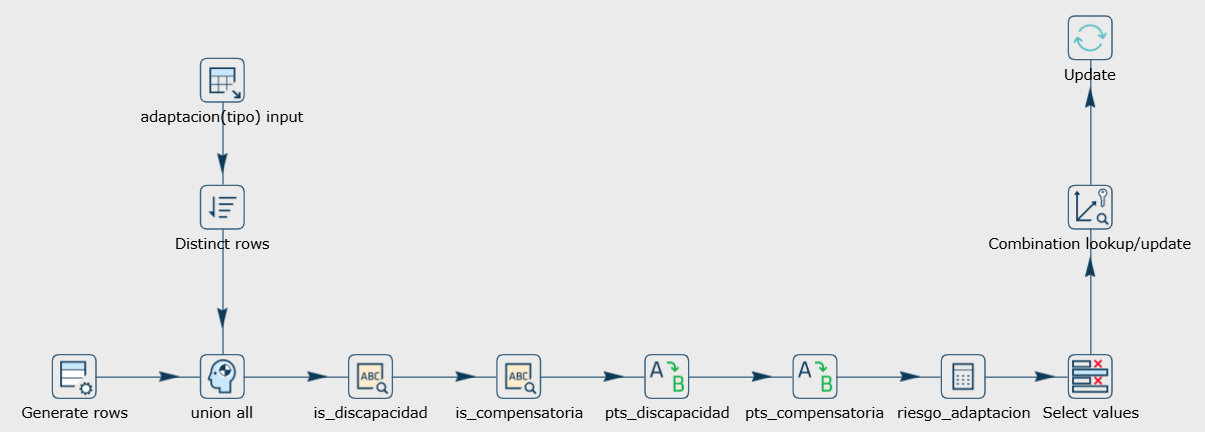
\includegraphics[width=0.85\textwidth]{imaxes/dim_adaptacion.png}
    \caption{Flujo del pipeline \textit{dim\_adaptacion.hpl}.}
    \label{fig:dim_adaptacion}
\end{figure}

\subsection{Dimensión de centro}

El pipeline de centro encapsula lógicas de limpieza para la geolocalización analítica. El campo \textit{direccion} se particiona mediante \textit{FieldSplitter}, se limpia el prefijo literario de los códigos postales (\textit{ReplaceString}) y se formatea al tipo numérico (\textit{SelectValues}) antes de generar la clave \textit{id\_centro} (ver figura \ref{fig:dim_centro}).

\begin{figure}[htbp]
    \centering
    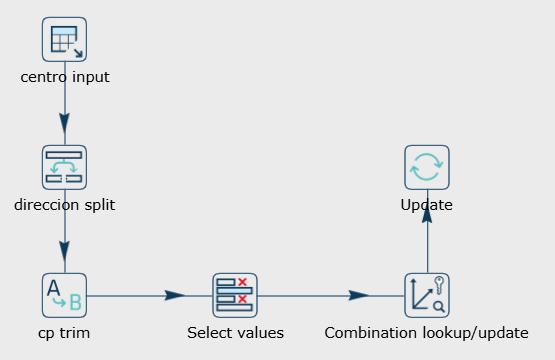
\includegraphics[width=0.85\textwidth]{imaxes/dim_centro.png}
    \caption{Flujo del pipeline \textit{dim\_centro.hpl}.}
    \label{fig:dim_centro}
\end{figure}

\subsection{Tabla de hechos de calificaciones}

Este es el pipeline central del sistema. Su objetivo es poblar la tabla de hechos atómica \textit{fact\_calificaciones}, cruzando los eventos transaccionales con todas las dimensiones construidas previamente y calculando métricas volátiles en el momento del evento (ver figura \ref{fig:fact_calificaciones_p1} y figura \ref{fig:fact_calificaciones_p2}).

\begin{enumerate}
    \item \textbf{Ingesta y cruce base (\textit{Table Input}, \textit{SortRows}, \textit{DBLookup}):} El flujo arranca extrayendo las calificaciones desde \textit{raw.linea\_expediente}, ordenándolas en memoria, y utilizando un nodo \textit{DBLookup} contra \textit{raw.matricula} para heredar metadatos vitales como la \textit{fecha} formal de matriculación, el \textit{curso\_academico} y el \textit{cod\_centro}.
    \item \textbf{Resolución de claves estáticas (\textit{DBLookup} en cascada):} A continuación, se encadenan cuatro nodos idénticos de tipo \textit{DBLookup} que interrogan a las dimensiones estáticas (\textit{dim\_asignatura}, \textit{dim\_centro}, \textit{dim\_curso} y \textit{dim\_tiempo}) cotejando las claves naturales para extraer sus identificadores subrogados. Críticamente, del nodo "\textit{dim\_curso lookup}" no solo se extrae la clave, sino que se arrastra la variable precalculada \textit{edad\_ideal}.
    \item \textbf{Resolución temporal SCD2 (\textit{Dimension Lookup}):} Para enlazar la dimensión del estudiante, se emplea un potente nodo \textit{Dimension Lookup} pasándole la \textit{fecha} de matrícula extraída en el primer paso. Hop coteja automáticamente esta fecha contra los atributos \textit{date\_from} y \textit{date\_to} de la dimensión, devolviendo el \textit{id\_estudiante} que encapsula la realidad familiar que tenía el alumno \textbf{en el momento exacto de matricularse}.
    \item \textbf{Cálculo algebraico de retraso académico (\textit{StringCut} y \textit{Calculator}):} Un nodo \textit{StringCut} extrae el año del \textit{curso\_academico}, y tres nodos \textit{Calculator} entran en juego: extraen el año de nacimiento, calculan la \textit{edad\_academica} del alumno en ese curso, y le restan la \textit{edad\_ideal} arrastrada de la dimensión curso para obtener matemáticamente la métrica \textit{desfase\_edad}.
    \item \textbf{Recálculo demográfico histórico (\textit{DBJoin} y \textit{Combination Lookup}):} Un nodo \textit{DBJoin} interroga la tabla de encuestas inyectando la restricción SQL fecha <= ? (usando la fecha de la matrícula) para rescatar la encuesta vigente en aquel momento. A partir de sus columnas crudas, se recalculan las unidades de consumo, la renta por consumo, y se infiere el \textit{riesgo\_socioeconomico}. Finalmente, el nodo avanzado \textit{CombinationLookup} mapea estos atributos contra \textit{dim\_demografia\_familiar} para asignar o crear el \textit{id\_demografia\_familiar}.
    \item \textbf{Carga incremental tipo Upsert (\textit{Insert / update}):} Superada la lógica de transformación, el pipeline utiliza un nodo transaccional \textit{Insert / update} para volcar los datos. Este componente evalúa si la combinación de claves ya existe: si existe, ejecuta una actualización (\textit{Update}) sobre las métricas; si es inédito, realiza una inserción limpia (\textit{Insert}). Este mecanismo asegura la persistencia del historial acumulado y es el pilar que da soporte a la arquitectura \textit{Change Data Capture (CDC)}.
\end{enumerate}

\begin{figure}[htbp]
    \centering
    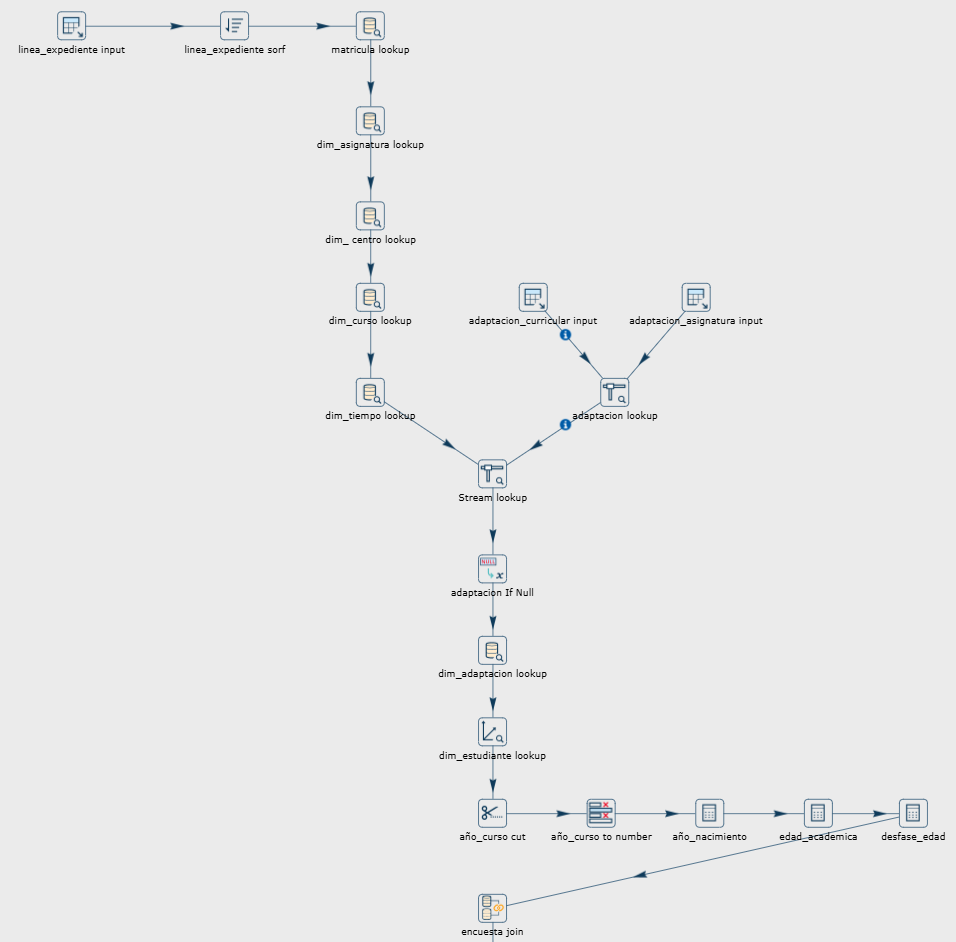
\includegraphics[width=0.85\textwidth]{imaxes/fact_calificaciones_p1.png}
    \caption{Flujo del pipeline \textit{fact\_calificaciones.hpl} (Parte 1).}
    \label{fig:fact_calificaciones_p1}
\end{figure}

\begin{figure}[htbp]
    \centering
    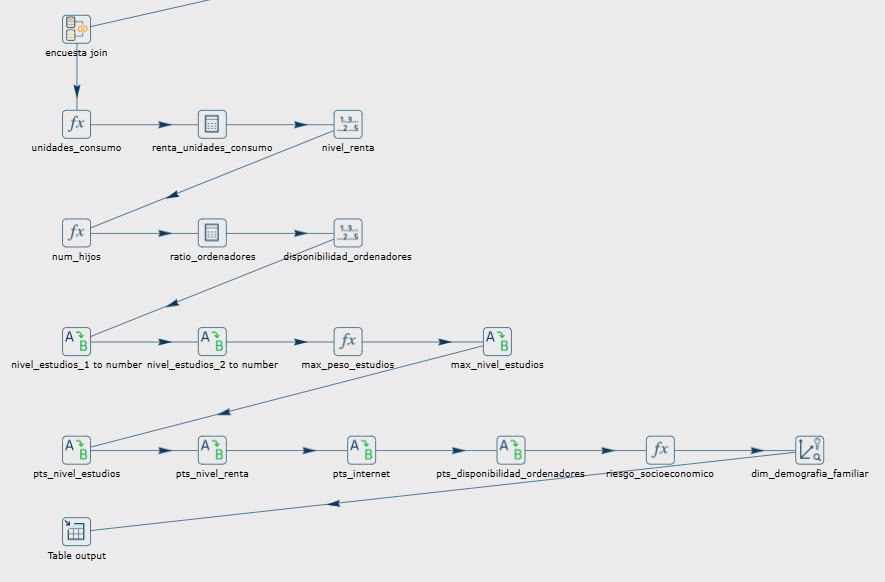
\includegraphics[width=0.85\textwidth]{imaxes/fact_calificaciones_p2.png}
    \caption{Flujo del pipeline \textit{fact\_calificaciones.hpl} (Parte 2).}
    \label{fig:fact_calificaciones_p2}
\end{figure}

\subsection{Tabla de hechos de rendimiento por evaluación}

El último proceso del ecosistema ETL actúa como el motor predictivo del proyecto, consolidando las calificaciones para calcular el riesgo final de abandono escolar. Para dotar al sistema de la capacidad de procesar recargas históricas completas y, al mismo tiempo, soportar un modo de ejecución por evaluación de alta eficiencia, este cálculo se ha dividido en dos pipelines paralelos: \textit{fact\_rendimiento\_anual\_full.hpl} y \textit{fact\_rendimiento\_anual\_incremental.hpl}.

\subsubsection{Lógica de consolidación masiva (pipeline full)}

Este pipeline (ver figuras \ref{fig:fact_rendimiento_anual_full_p1} y figura \ref{fig:fact_rendimiento_anual_full_p2}) abandona la clásica consolidación estática anual y adopta una arquitectura de "Suma Acumulada" manteniendo el grano de la tabla a nivel de Evaluación (\textit{id\_estudiante} $\times$ \textit{id\_tiempo}).

\begin{enumerate}
    \item \textbf{Ingesta y tipificación analítica (\textit{Formula}):} Tras ingerir los datos y cruzar con las dimensiones, un nodo \textit{Formula} bautizado como ``flags analíticos'' perfila las casuísticas de cada nota. Es aquí donde se detecta de forma temprana si el registro pertenece al ciclo crítico de 1.º y 2.º de primaria, y se despliegan vectores binarios para segmentar si un suspenso es parcial o final.
    \item \textbf{Rastreo histórico acumulado (flujo principal):} Tras una ordenación cronológica estricta, un nodo \textit{Group By} agrupa por estudiante activando la directiva \textit{"Include all rows"}. Implementando funciones \textit{Cumulative sum} sobre los vectores previamente generados, el sistema emula una \textit{Window Function}. Esto arrastra en el registro actual todo el bagaje histórico de suspensos segmentados del alumno.
    \item \textbf{Motor detección de repetidores (sub-rama paralela):} El flujo se bifurca hacia una rama auxiliar. Un nodo \textit{Analytic Query} (LAG 1) lee el \textit{curso\_anterior} del alumno, y una fórmula detecta matemáticamente la repetición. Un \textit{Group By} con sumatoria acumulativa calcula el cómputo histórico de repeticiones, y un \textit{StreamLookup} vuelve a inyectar este bagaje al flujo principal.
    \item \textbf{Ecuación maestra de riesgo (\textit{Formula}):} Un potente nodo de fórmulas convierte todas las acumulaciones en puntuaciones predictivas (Scoring). El \textbf{riesgo académico} se calcula ponderando de manera asimétrica los factores: suspensos finales en 1.º/2.º de primaria (20 pts), suspensos parciales (10 pts) y penalizando drásticamente la repetición en este ciclo temprano (40 pts). A la par, evalúa el riesgo base familiar creando una puntuación escalonada para el \textbf{riesgo socioeconómico} (10 pts si supera el umbral severo).
    \item \textbf{Cálculo del indicador de abandono (\textit{Calculator}):} Como culminación, un nodo sumatorio simple consolida matemáticamente el \textit{riesgo\_academico}, el \textit{riesgo\_adaptacion} y los puntos socioeconómicos, arrojando el indicador definitivo \textit{riesgo\_abandono}.
\end{enumerate}

\subsubsection{Adaptaciones del pipeline incremental}

El flujo \textit{Full} requiere volcar en RAM todo el historial autonómico, algo insostenible para recargas periódicas. La variante \textit{Incremental} (ver figura \ref{fig:fact_rendimiento_anual_incremental} y figura \ref{fig:fact_rendimiento_anual_incremental_join}) resuelve esto leyendo solo las notas del \textit{\$\{CURSO\_ACTUAL\}}.

Al no disponer del historial en memoria, utiliza un \textit{Database Join} contra la propia tabla destino para recuperar el \textit{riesgo\_academico} consolidado del año anterior. Como el modelo es aditivo, suma los puntos del año en curso al riesgo histórico extraído. Finalmente, emplea \textit{Insert / update} para inyectar los nuevos cálculos sin destruir el historial previo.

\begin{figure}[htbp]
    \centering
    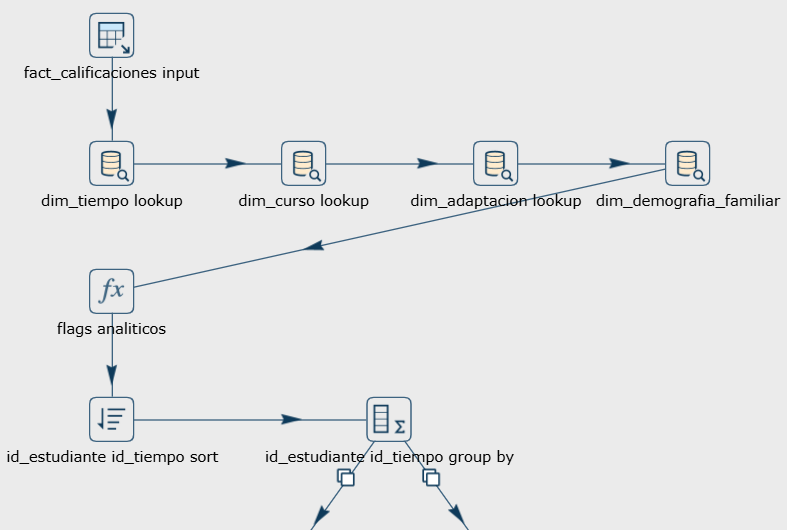
\includegraphics[width=0.85\textwidth]{imaxes/fact_rendimiento_anual_full_p1.png}
    \caption{Flujo del pipeline \textit{fact\_rendimiento\_anual\_full.hpl} (Parte 1).}
    \label{fig:fact_rendimiento_anual_full_p1}
\end{figure}

\begin{figure}[htbp]
    \centering
    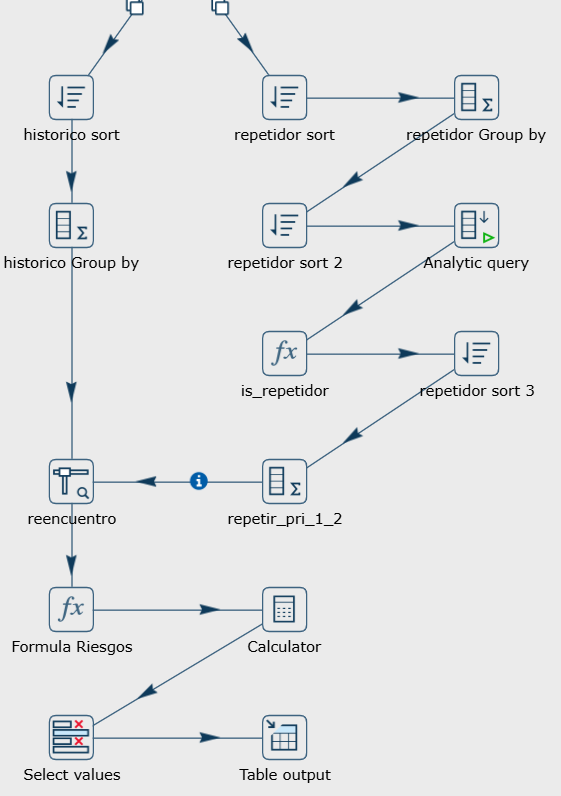
\includegraphics[width=0.85\textwidth]{imaxes/fact_rendimiento_anual_full_p2.png}
    \caption{Flujo del pipeline \textit{fact\_rendimiento\_anual\_full.hpl} (Parte 2).}
    \label{fig:fact_rendimiento_anual_full_p2}
\end{figure}

\begin{figure}[htbp]
    \centering
    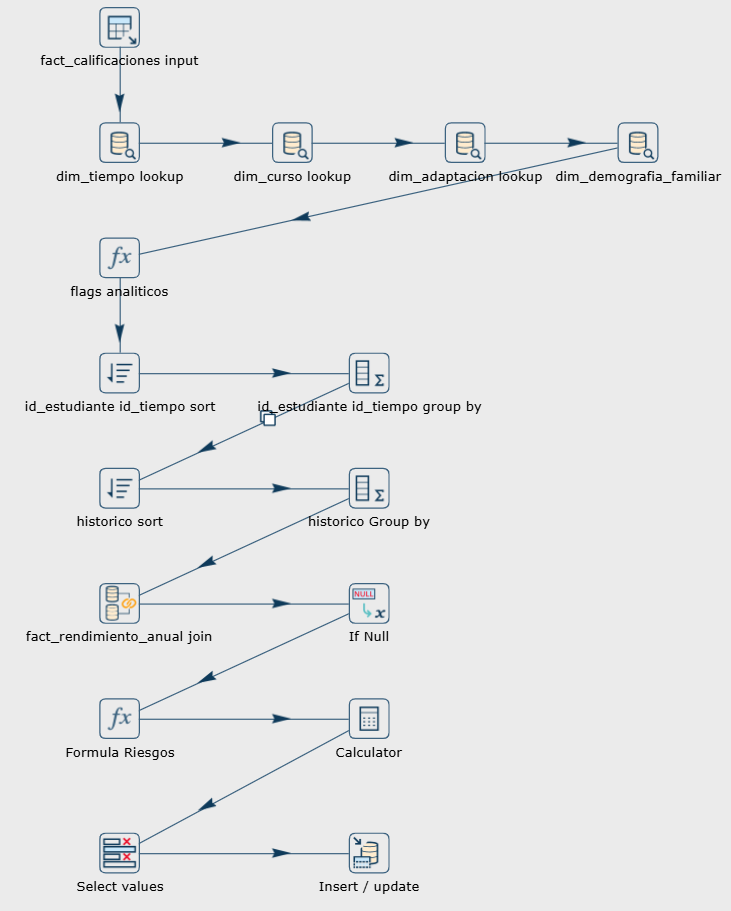
\includegraphics[width=0.85\textwidth]{imaxes/fact_rendimiento_anual_incremental.png}
    \caption{Flujo completo del pipeline \textit{fact\_rendimiento\_anual\_incremental.hpl}.}
    \label{fig:fact_rendimiento_anual_incremental}
\end{figure}

\begin{figure}[htbp]
    \centering
    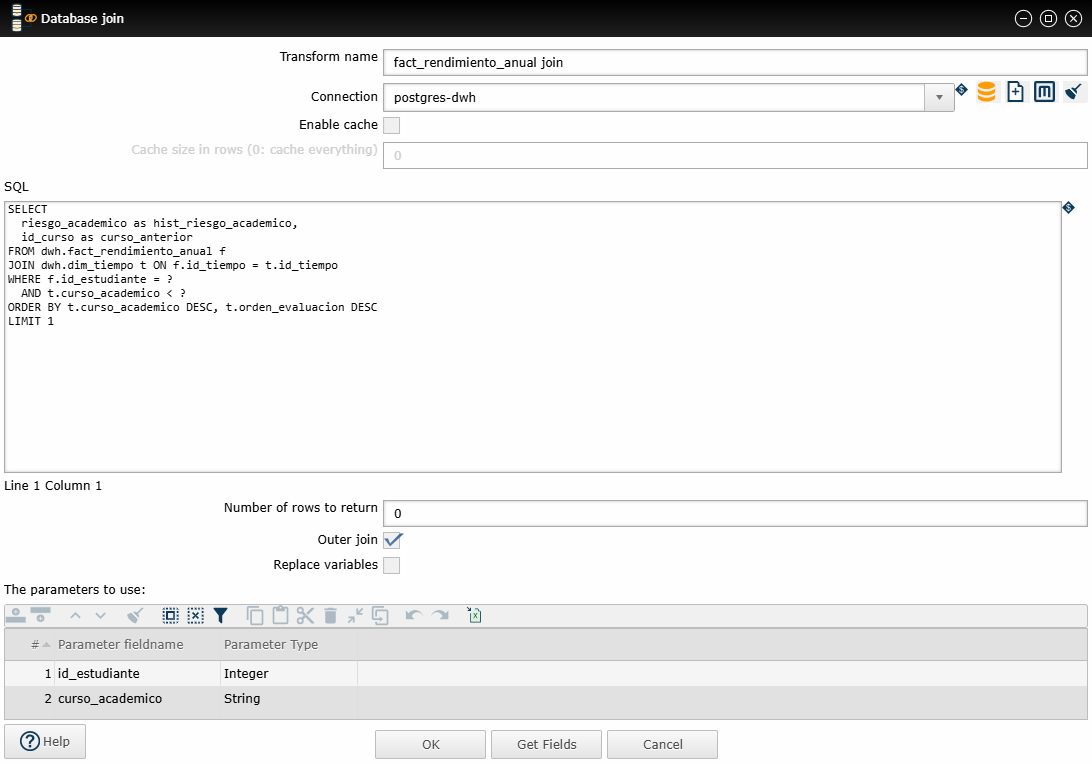
\includegraphics[width=0.85\textwidth]{imaxes/fact_rendimiento_anual_incremental_join.png}
    \caption{Nodo \textit{Database Join} en \textit{fact\_rendimiento\_anual\_incremental.hpl}.}
    \label{fig:fact_rendimiento_anual_incremental_join}
\end{figure}

\section{Orquestación y workflows}

Los pipelines son secuenciados por flujos de trabajo (\textit{Workflows}). La orquestación sigue una arquitectura jerárquica encabezada por \textit{main.hwf} (ver figura \ref{fig:main_workflow}), que delega en dos sub-workflows:

\begin{itemize}
    \item \textbf{\textit{dimensions.hwf}:} Extrae datos a \textit{Staging} y luego lanza en paralelo la carga de todas las dimensiones para maximizar el rendimiento (ver figura \ref{fig:dimensions_workflow}).
    \item \textbf{\textit{facts.hwf}:} Ejecuta secuencialmente las tablas de hechos. Un nodo \textit{Simple Evaluation} inspecciona el parámetro dinámico \textit{\$\{CURSO\_ACTUAL\}}: si está vacío, enruta hacia el pipeline \textit{Full}; si contiene un curso, enruta hacia el \textit{Incremental} (ver figura \ref{fig:facts_workflow}).
\end{itemize}

El parámetro \textit{CURSO\_ACTUAL} fluye en cascada desde la ejecución externa (Docker) hasta el código SQL de los pipelines, permitiendo que todo el ecosistema adapte su comportamiento a un nuevo año académico alterando un único valor.

La robustez se garantiza mediante un manejo de errores multinivel: si un pipeline individual falla, el sub-workflow detiene la ejecución, registra el error y lanza un \textit{Abort workflow} que se propaga jerárquicamente hasta abortar la orquestación global, previniendo cargas parciales o corruptas.

\begin{figure}[htbp]
    \centering
    
\includegraphics[width=0.85\textwidth]{imaxes/main_workflow.png}
    \caption{Workflow principal (\textit{main.hwf}) y delegación jerárquica.}
    \label{fig:main_workflow}
\end{figure}

\begin{figure}[htbp]
    \centering
    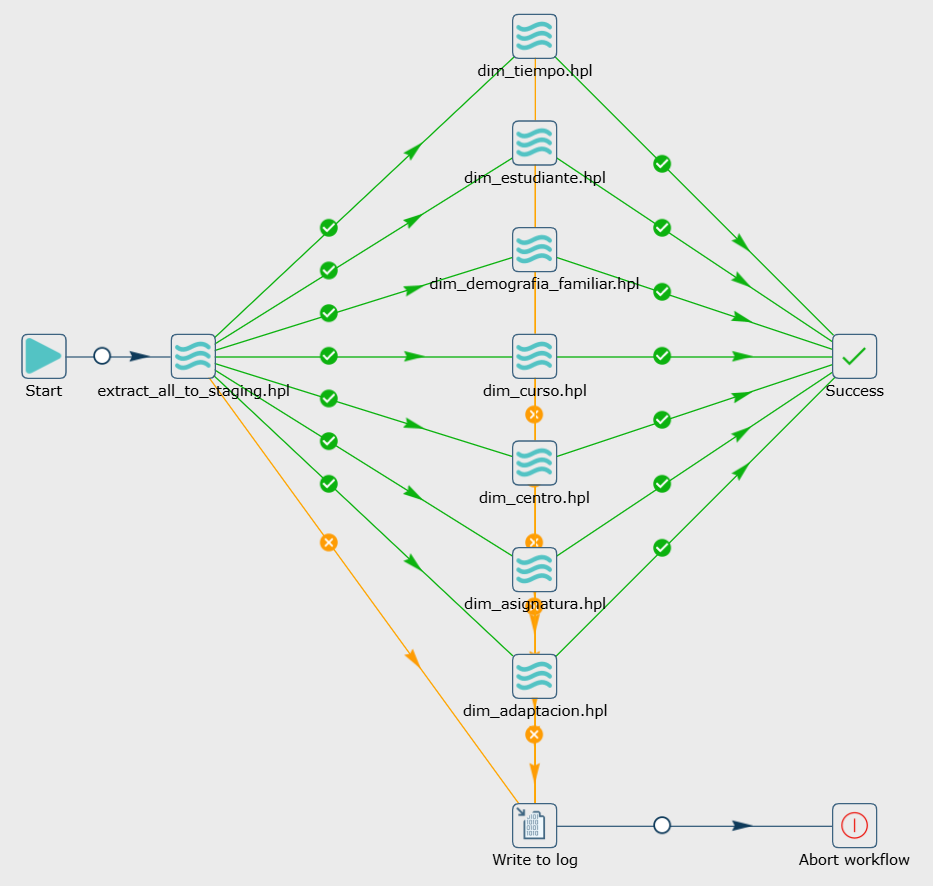
\includegraphics[width=0.85\textwidth]{imaxes/dimensions_workflow.png}
    \caption{Sub-flujo de dimensiones (\textit{dimensions.hwf}) en paralelo.}
    \label{fig:dimensions_workflow}
\end{figure}

\begin{figure}[htbp]
    \centering
    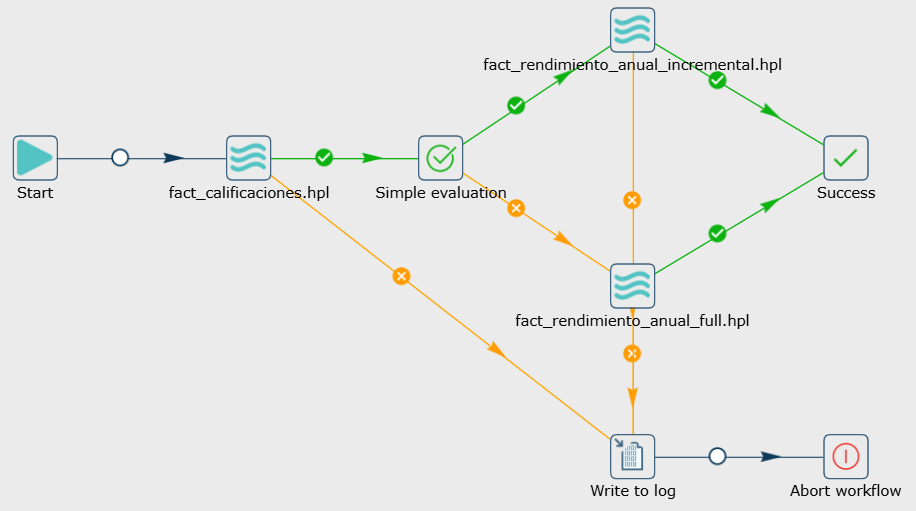
\includegraphics[width=0.85\textwidth]{imaxes/facts_workflow.png}
    \caption{Sub-flujo de hechos (\textit{facts.hwf}) ejecutado de forma secuencial.}
    \label{fig:facts_workflow}
\end{figure}
